\documentclass{article}
\usepackage[utf8]{inputenc}
\usepackage{amsmath}
\usepackage{graphicx}
\usepackage{hyperref}
\parindent=0pt
\usepackage[a4paper, total={165mm, 235mm}]{geometry}
\usepackage[section]{placeins}
\usepackage{enumitem}
\usepackage{caption}
\usepackage{parskip}
\usepackage{multirow}
\usepackage{biblatex}
\addbibresource{Bibliography.bib}
\usepackage{wrapfig}

\title{PySPI for Persistent Sources}
\author{Möller, Julius}
\date{June 2023}

\begin{document}

\begin{titlepage}
    
    
\includegraphics[height=1cm]{Images/General/MPE_logo_189x180px.jpg}
    \hfill
    
\includegraphics[height=1cm]{Images/General/PH.pdf}
    
\includegraphics[height=1cm]{Images/General/tumlogo.pdf}

    \begin{center}
        \vspace{1cm}
        \large

        Max Planck Institute for Extraterrestrial Physics
        

        \vspace{1.5cm}
        \large
        Thesis for Master of Science in Astrophysics
        
        \vspace{3cm}
        \Huge
        PySpi for Persistent Sources
        
        \vspace{3cm}
        
        \LARGE
        Julius Möller
        
        \vspace{1.5cm}
        \large
        June 2023
        
        
        \vspace{6.5cm}
        
        
        
        \large
        Technische Universität München

        Fakultät für Physik
        
        
        
    \end{center}
\end{titlepage}


\tableofcontents

\pagebreak

\section{About INTEGRAL}




The INTErnational Gamma-Ray Astrophysics Laboratory (INTEGRAL) is an ESA space telescope with contributions from NASA and the RKA. Its mission began on October 17, 2002, when a Proton-DM2 rocket launched it from the Russian Baikonur spaceport in Kazakhstan into a 3-day, highly elliptical orbit with an apogee of 153000km and a perigee of 9000km, although this has not remained constant over the course of its lifetime. This places INTEGRAL mostly above radiation belts that would cause high instrumental backgrounds from charged-particle activation, and is why data collecting is halted during hours of close Earth-proximity. Initially, INTEGRAL had a 2+3-year planned lifetime, which it has greatly exceeded due to its lower than expected fuel consumption. Since then, its science operations have been repeatedly extended, currently up to the end of 2024, with some difficulties along the way such as its failed thrusters in July 2020 (compensated through the use of reaction wheels) and an uncontrolled tumbling caused by a single event upset in September 2021. The satellite is predicted to reenter Earth's atmosphere in 2029.

Onboard INTEGRAL are two main instruments: the Imager on-Board the INTEGRAL Satellite (IBIS) and the SPectrometer of INTEGRAL (SPI). IBIS specializes in being able to locate sources effectively. With an angular resolution of 12 arcmin, it can locate bright sources with arcmin precision in its $9^\circ \times 9^\circ$ field of view, and covers an energy range from 15keV to 10MeV. 

\subsection{About SPI}

\begin{wrapfigure}{r}{0.55\textwidth}
    \begin{center}
      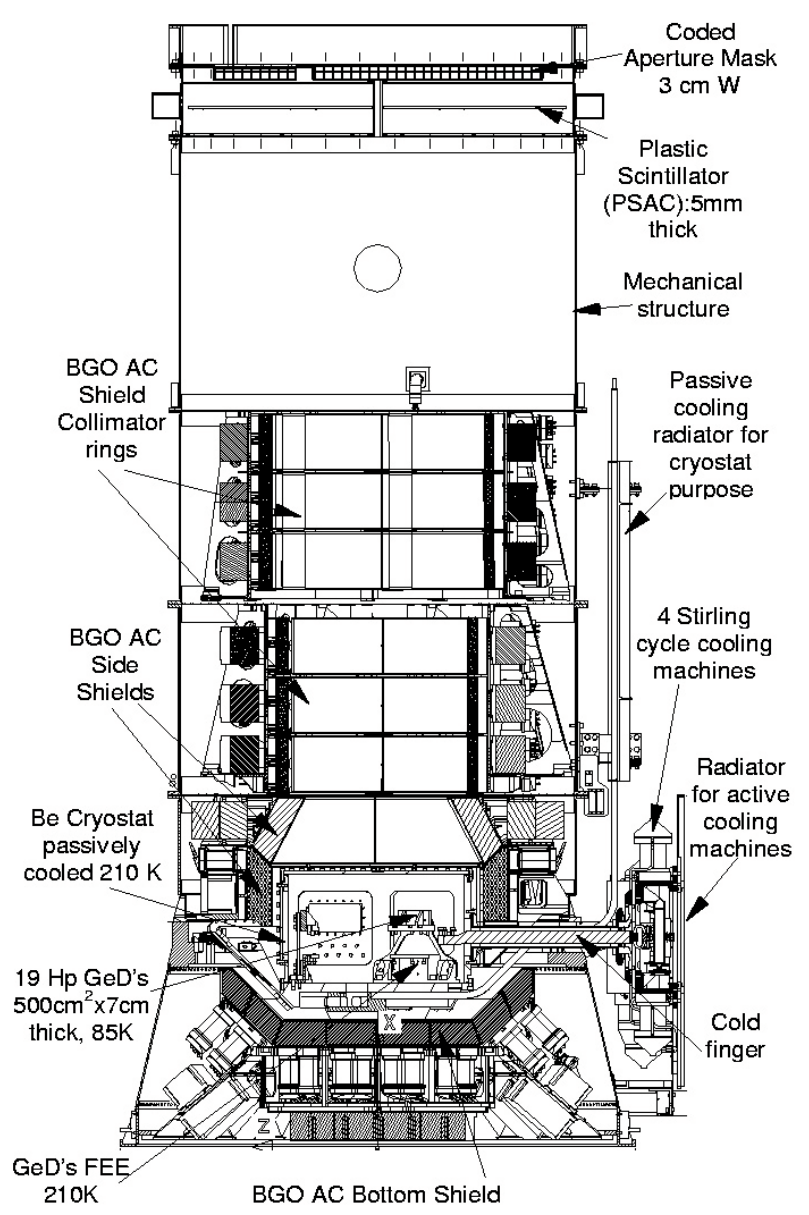
\includegraphics[width=0.53\textwidth]{Images/General/SPI_cut_view_verdenne_2003.PNG}
    \end{center}
    \caption{Cut-out view of the SPI spectrometer \cite{refId0}.}
    \label{SPI cut view}
\end{wrapfigure}




SPI, the instrument used in this Thesis and illustrated in figure \ref{SPI cut view}, specializes in its detailed energy resolution. It 1.3MeV, it is able to resolve energies with 2.5keV precision. At has a field of view of $16^\circ$ and an energy range covering 20keV to 8MeV.

\subsubsection*{Detectors}
SPIs detectors are composed of an hexagonal array of 19 reverse-electrode n-type germanium detectors. With a mean crystal weight of 951g and mean volume of $178\text{cm}^3$, the total geometrical area for a flux parallel to the axis is $178\text{cm}^2$. Under normal working conditions, a voltage of 4000V is applied to each detector independently, and this voltage is variable between zero and 5000V. The germanium detectors require temperatures below 100K to work effectively, preferably as low as 85K in order to slow the effects of radiation damage. To accomplish this, INTEGRAL is equipped with an active cryogenic system. The Ge array is fixed on a Be plate, which is placed inside the cryostat. The plate is connected to the Stirling cycle cryocoolers to provide active cooling. 

\subsubsection*{Mask}
\begin{wrapfigure}{l}{0.35\textwidth}
    \begin{center}
      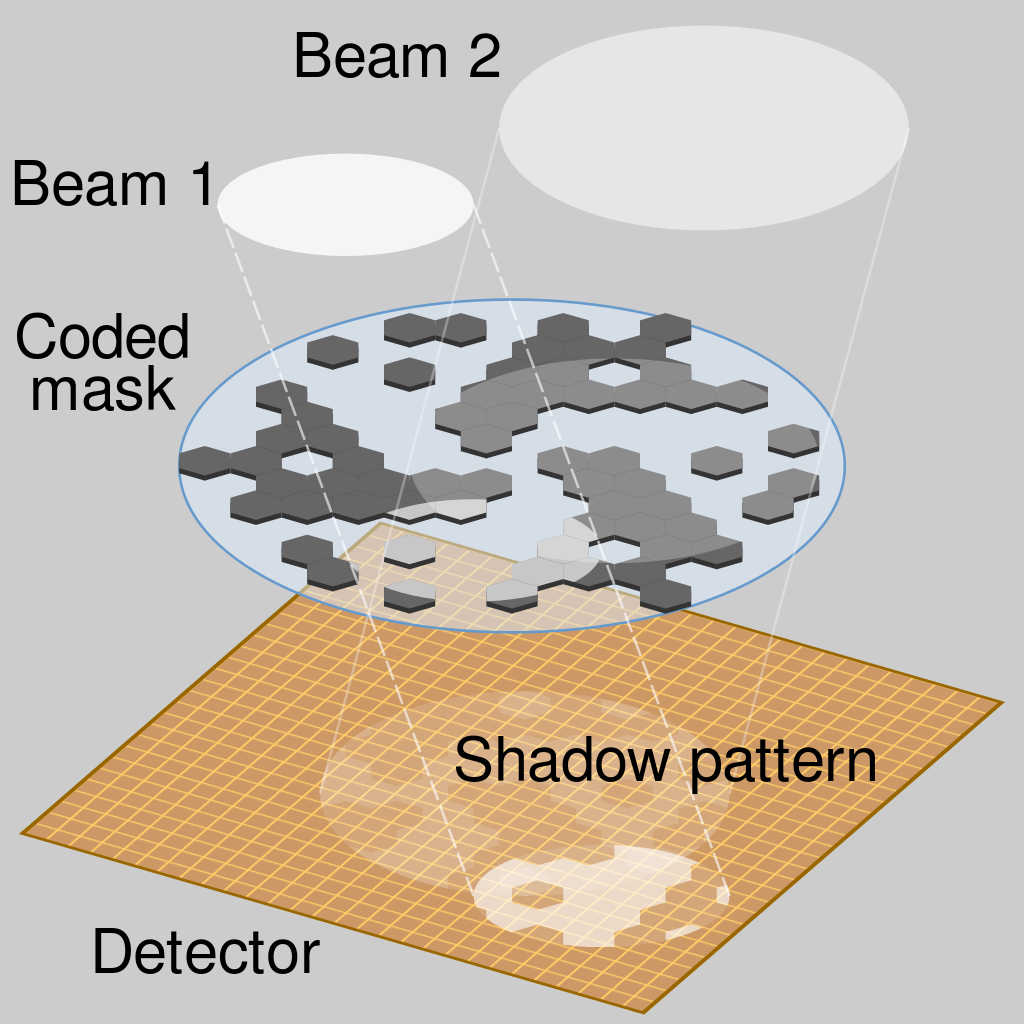
\includegraphics[width=0.33\textwidth]{Images/General/HURA_hexagonal_coded_aperture_mask_principle.svg.png}
    \end{center}
    \caption{\cite{HURA}.}
    \label{HURA}
\end{wrapfigure}

Before any photons can reach the array of detectors, they must pass through the coded aperture mask made of a 3cm thick tungsten alloy, located 1.71m above. The $120^\circ$ rotationally symmetric mask is composed of 127 hexagonal tiles (63 opaque and 64 transparent to gamma radiation in the operating energy range) measuring 60mm side to side, and is inscribed within a circle with 720mm diameter. The effect that the mask has on incoming source beams is illustrated in figure \ref{HURA}. The complex shadow patterns created on the detector array allows one to infer the position of measured sources.







\section{Test}

\pagebreak

adf

\pagebreak

\nocite{*}
\printbibliography



\end{document}